% Copyright (c) 2022 Tobias Briones. All rights reserved.
%
% SPDX-License-Identifier: CC-BY-SA-4.0
%
% This file is part of Course Project at UNAH-IS911: Microprocessors.
%
% This source code is licensed under the Creative Commons Attribution Share
% Alike 4.0 International License found in the LICENSE file in the root
% directory of this source tree or at https://spdx.org/licenses/CC-BY-SA-4.0.

\documentclass[conference]{IEEEtran}
\usepackage[letterpaper, portrait, margin=2cm]{geometry}
\usepackage[style=ieee]{biblatex}
\usepackage[utf8]{inputenc}
\usepackage[spanish]{babel}
\usepackage{geometry}
\usepackage[]{graphics}
\usepackage[demo]{graphicx}
\usepackage{csquotes}
\usepackage{float}
\usepackage{hyperref}
\usepackage[table,xcdraw]{xcolor}
\usepackage{lipsum}
\usepackage{dirtytalk}
\usepackage{listings}

\addbibresource{bibliography.bib}

\title{Microcontrolado PIC}
\author{
    
\includegraphics[width = 40mm]{images/logo-unah.png}\\[8ex]
    \IEEEauthorblockN{Tobias Briones}
    \IEEEauthorblockN{tobias.briones@unah.hn}
    \IEEEauthorblockA{\textit{Universidad Nacional Autónoma de Honduras} \\
    \textit{Ingeniería de Sistemas} \\
    \textit{I PAC 2022} \\
    \textit{IS911-MICROPROCESADORES}} \\\vspace*{20pt} \normalsize  \\
    \today
}

\hypersetup{
    colorlinks=true,
    linkcolor=black,
    filecolor=magenta,
    urlcolor=cyan,
    citecolor=black
}

\newcommand\blfootnote[1]{%
    \begingroup
    \renewcommand\thefootnote{}\footnote{#1}%
    \addtocounter{footnote}{-1}%
    \endgroup
}

\definecolor{codegreen}{rgb}{0,0.6,0}
\definecolor{codegray}{rgb}{0.5,0.5,0.5}
\definecolor{codepurple}{rgb}{0.58,0,0.82}
\definecolor{backcolour}{rgb}{0.95,0.95,0.92}

\lstdefinestyle{mystyle}{
    backgroundcolor=\color{backcolour},
    commentstyle=\color{codegreen},
    keywordstyle=\color{magenta},
    numberstyle=\tiny\color{codegray},
    stringstyle=\color{codepurple},
    basicstyle=\ttfamily\footnotesize,
    breakatwhitespace=false,
    breaklines=true,
    captionpos=b,
    keepspaces=true,
    numbers=left,
    numbersep=5pt,
    showspaces=false,
    showstringspaces=false,
    showtabs=false,
    tabsize=2
}

\lstset{style=mystyle}

\begin{document}

    \maketitle

    \begin{abstract}
        En esta investigación se presenta un resumen sobre los
        microcontroladores PIC orientado a la gama de entrada PIC16 así como
        un ejemplos en lenguaje ensamblador y lenguaje C para adentrarse un
        poco en estos dispositivos.
    \end{abstract}

    \tableofcontents

    \blfootnote{
        Copyright (c) 2022 Tobias Briones. All rights reserved. \\
        This work is licensed under the Creative Commons Attribution Share
        Alike 4.0 International License (\href{https://spdx
.org/licenses/CC-BY-SA-4.0}{CC-BY-SA-4.0}). \\
        Third party contents available under their respective copyright and
        license.\\
        For more details go to the \href{https://github
.com/tobiasbriones/cp-unah-is911-microprocessors}{GitHub Repository}.}

    \section{Introducción}

    Los PIC son una familia de microcontroladores desarrollados por Microchip
    Technologies \cite{microchip-technology-inc-2013} los cuales son muy
    conocidos y utilizados tanto a nivel educativo como industrial.
    Cualquiera que está interesado en el aprendizaje o implementación de
    circuitos electrónicos, IoT o sistemas embebidos definitivamente debió de
    haber conocido o utilizado estos microcontroladores ya que son tan
    populares como las tarjetas Arduino. Así mismo, tienen una gran historia
    por detrás que data desde el año $1976$ y según wikipedia tenemos que
    \cite{wikipedia-pic-2022}:

    \bigbreak

    \begin{quote}
        \textbf{PIC} (generalmente pronunciado como "pick") es una familia de
        microcontroladores fabricados por Microchip Technology, derivados del
        PIC1650 desarrollado originalmente por la División de Microchip de
        General Instrument (GI). El nombre PIC inicialmente se refería a
        Controlador de Interfaz Periférico, y actualmente se expande como
        Computadora Inteligente Programable. Las primeras partes de la
        familia estuvieron disponibles en 1976; en 2013, la empresa había
        enviado más de doce mil millones de piezas individuales, utilizadas
        en una amplia variedad de sistemas integrados.
        \\
        \small Fuente: Wikipedia $\mid$ PIC microcontrollers (traducido de
        inglés a español) \cite{wikipedia-pic-2022}
    \end{quote}

    Los PICs han evolucionado en el tiempo. Por ejemplo, algunos modelos
    iniciales usaban la ROM directamente (o como se dice hard-coded o
    hard-written) para almacenar el código pero luego los modelos actuales
    empezaron a utilizar EPROM y EEPROM, ahora memoria flash y por último el
    PIC permite que se reprograme solo \cite{wikipedia-pic-2022}. Esto
    implica una gran ventaja para el programador humano.

    \bigbreak

    El IDE que utilizan los PICs es un software propietario del proveedor
    Microchip Technologies el cual permite lenguaje ensamblador y C/C++
    \cite{microchip-technology-inc-2013} \cite{wikipedia-pic-2022}. Aunque
    otros lenguajes de bajo nivel como Rust \footnote{A veces causa polémica
    decir que un lenguaje es de bajo nivel. Yo lo defino como tomar el
    subconjunto (unsafe) del lenguaje que lo hace de bajo nivel (o framework
    de ensamblador) o simplemente referirse como \say{lenguaje de más bajo
    nivel}.} también se pueden emplear para programar dispositivos sin
    sistema operativo (\say{el metal}) pero hay que tener en cuenta que puede
    haber falta de soporte para las arquitecturas de CPU y compiladores u
    otras herramientas.

    \bigbreak

    \begin{figure}[H]
        \centering
        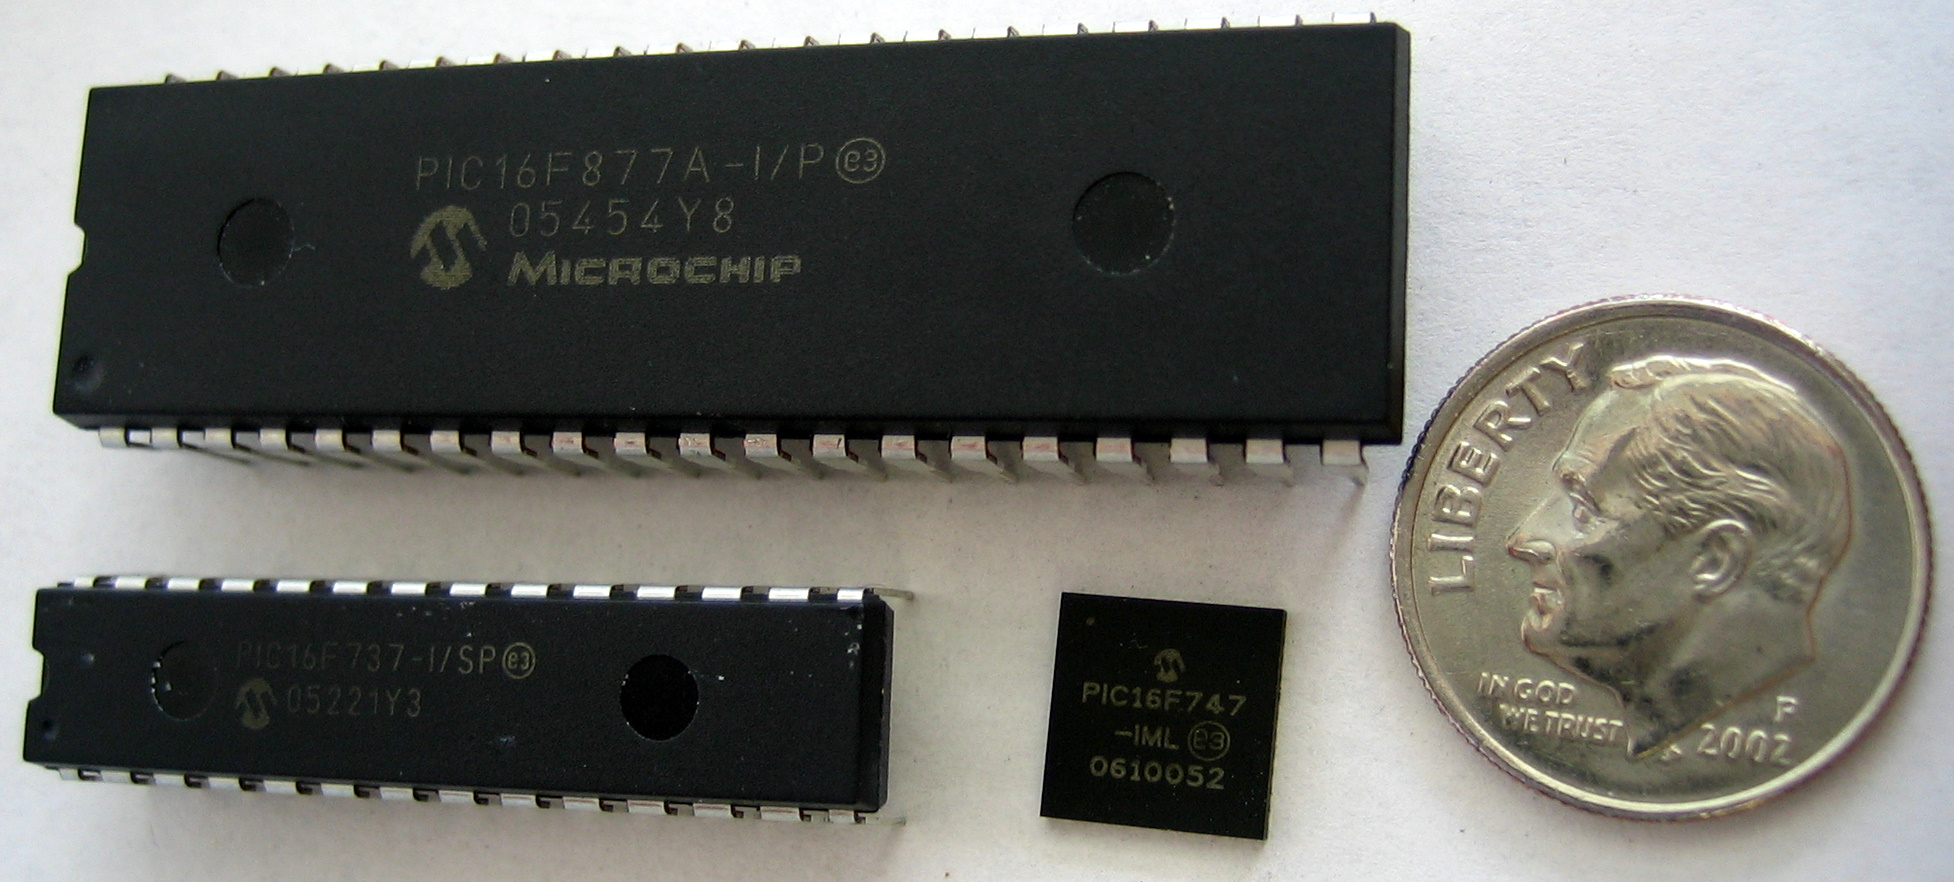
\includegraphics[width=0.3\paperwidth]{images/pic-microcontrollers.jpg}
        \caption{Microcontroladores PIC} \footnotesize
        Fuente: Wikipedia $\mid$ Por MikeMurphy, dominio público,
        https://commons.wikimedia.org/w/index.php?curid=1225813
        \cite{wikipedia-pic-2022}
    \end{figure}

    \subsection{Familia de PICs de Entrada}

    Con respecto a la familia $16$ reconocida como número $10Fxxx$, $12Fxxx$,
    y $16Fxxx$ de los PIC tenemos que es una gama de entrada que utiliza
    palabras de $12-bit$ y funciona de forma que sea económica y funcional
    con una arquitectura de $8-bit$ y poseen
    \cite{microchip-developer-help-2022}.

    \bigbreak

    \begin{itemize}
        \item Simplicidad para desarrollo con conjunto de instrucciones de
        \item $33$ ($12-bit$ de ancho).
        \item Palabra de $2K$ ($3KB$) de memoria de programación direccionable.
        \item RAM de máximo $144bytes$.
        \item Hardware de 2 niveles.
        \item Un registro ($8-bit$) de registro de selección.
        \item Fácil migración y opciones de producto.
        \item Factores de forma más pequeños posible.
    \end{itemize}

    \bigbreak

    \begin{figure}[H]
        \centering
        \includegraphics[width=0.3\paperwidth]{images/microchip-pic16c58a.jpg}
        \caption{Microcontrolador PIC 16C58A} \footnotesize
        Fuente: Wikipedia $\mid$ By © Raimond Spekking / CC BY-SA 4.0 (via
        Wikimedia Commons), CC BY-SA 4.0, https://commons.wikimedia
        .org/w/index.php?curid=75910927 \cite{wikipedia-pic-2022}
    \end{figure}

    \bigbreak

    En el año $1,998$ Microchip introdujo el PIC 16F84 el cual ya tenía
    memoria flash programable y borrable, sin embargo, el modelo PIC16C84
    introducido en $1,993$ fue el primero con memoria EEPROM
    \cite{wikipedia-pic-2022}.

    \bigbreak

    Asimismo, con respecto a la versión F específicamente se sabe que:

    \bigbreak

    \begin{quote}
        El PIC16F84/PIC16F84A es una versión mejorada del PIC16C84, y casi
        completamente compatible, con mejor seguridad de programa y usando
        memoria flash en lugar de memoria EEPROM para la memoria del programa
        . El PIC16F84/PIC16F84A tiene 68 bytes de RAM mientras que el
        PIC16C84 tiene 36 bytes.\\
        \small Fuente: Wikipedia $\mid$ PIC16x84 (traducido de inglés a
        español) \cite{wikipedia-pc16x84-2020}
    \end{quote}

    \subsection{Atributos del PIC 16F84}

    Entre las características comerciales actualmente encontradas en
    \textit{Mouser Electronics} -Tienda de gran variedad de semiconductores y
    componentes electrónicos en el mundo- tenemos:

    \bigbreak

    \begin{table}[H]
        \centering
        \begin{tabular}{|l|l|}
            \hline
            \rowcolor[HTML]{CBCEFB}
            \textbf{Atributo}          & \textbf{Valor}                  \\
            \hline
            Fabricante                 & Microchip                       \\
            \hline
            \rowcolor[HTML]{EFEFEF}
            Categoría                  & Microcontrolador de 8bits - MCU \\
            \hline
            RoHS                       & Si                              \\
            \hline
            \rowcolor[HTML]{EFEFEF}
            Serie                      & PIC16(L)F8x                     \\
            \hline
            Tipo de montaje            & SMD/SMT                         \\
            \hline
            \rowcolor[HTML]{EFEFEF}
            Paquete                    & SOIC-18                         \\
            \hline
            Núcleo                     & PIC16                           \\
            \hline
            \rowcolor[HTML]{EFEFEF}
            \begin{tabular}[c]{@{}l@{}}
                Tamaño de memoria \\ del programa
            \end{tabular} & 1.75kB \\ \hline
            \begin{tabular}[c]{@{}l@{}}
                Ancho de banda\\ del bus de datos
            \end{tabular}             & 8bit                           \\ \hline
            \rowcolor[HTML]{EFEFEF}
            Frecuencia de reloj máxima     & 10MHz
            \\ \hline
            Número de I/Os       & 13I/O                         \\ \hline
            \rowcolor[HTML]{EFEFEF}
            Tamaño de RAM de datos & 68B \\ \hline
            Voltaje de operación                       & 2V a 6V
            \\ \hline
            \rowcolor[HTML]{EFEFEF}
            \begin{tabular}[c]{@{}l@{}}
                Min.-Máx Temperatura \\ de operación
            \end{tabular}                      & 0C hasta +70C
            \\ \hline
            Alto            & 2.31mm                      \\ \hline
            \rowcolor[HTML]{EFEFEF}
            Longitud            & 11.53mm                      \\ \hline
            Ancho            & 7.49mm                      \\ \hline
            \rowcolor[HTML]{EFEFEF}
            Peso por unidad            & 0.007408oz                      \\
            \hline
        \end{tabular}
        \caption{Especificaciones comerciales del PIC16F84-10/SO} \footnotesize
        Fuente: PIC16F84-10/SO Microchip Technology $\mid$ Mouser
        \cite{mouser-electronics-inc-2022}
    \end{table}

    \bigbreak

    Para mayor detalle técnico sobre el PIC16F8X (notar que X es un comodín)
    se encuentra como de costumbre la hoja de especificaciones oficial del
    dispositivo \cite{microchip-technology-pic16f8x-2013} que el lector puede
    leer pero también tener en cuenta el modelo a adquirir al momento de la
    compra como lo describe la tabla de arriba.

    \section{Programa en Ensamblador}

    En esta sección se provee un programa básico para PIC16F84 que enciende y
    apaga un LED tomado de \textit{PIC Programming in
    Assembly}\cite{mit-no-date}.

    \bigbreak

    \begin{lstlisting}[language={[x86masm]Assembler}, caption=Programa en
    ensamblador para PIC16F84 que enciende y apaga un LED]
; PIC Programming in Assembly at http://groups.csail.mit
.edu/lbr/stack/pic/pic-prog-assembly.pdf

; Definir las constantes
STATUS equ 03h ;Direccion del registro para STATUS
TRISA equ 85h ;Direccion del registro TRISTATE para el puerto A
PORTA equ 05h ;Direccion del puerto A
COUNT1 equ 08h ;Primer contador para el retraso de los loops
COUNT2 equ 09h ;Segundo contador para el retraso de los loops

; Configurar el puerto
    bsf STATUS,5 ; Cambiar al Banco 1
    movlw 00h ; Hacer los pines del puerto A
    movwf TRISA ; Para la salida
    bcf STATUS,5 ; Cambiar  de regreso al Banco 0

; Encender el LED
Start   movlw 02h ; Encender el LED poniendolo en el
        movwf PORTA ; registro w y luego en el puerto

; Empezar el retraso del loop 1
Loop1 decfsz COUNT1,1 ; Restar 1 de 255
      goto   Loop1 ; Si COUNT es cero, continuar
      decfsz COUNT2,1 ; Restar 1 de 255
      goto   Loop1 ; Regresar al inicio del loop
                    ; Este retraso cuenta atras desde
                    ; 255 a cero, 255 veces

; Retraso terminado, ahora apagar el LED
    movlw   00h ; Apagar el LED poniendolo en el registro
    movwf   PORTA ; w y entonces en el puerto

; Agragar otro retraso
Loop2   decfsz COUNT1,1 ; Mantiene el LED apagado
        goto Loop2 ; lo suficiente para notarlo
        decfsz COUNT2,1
        goto Loop2

; Ir al inicio del programa
    goto Start ; Ir al inicio y encender
                 el LED de nuevo

end ; requerido por algunos comp.
    \end{lstlisting}

    \bigbreak

    El circuito para probar este código es el siguiente:

    \bigbreak

    \begin{figure}[H]
        \centering
        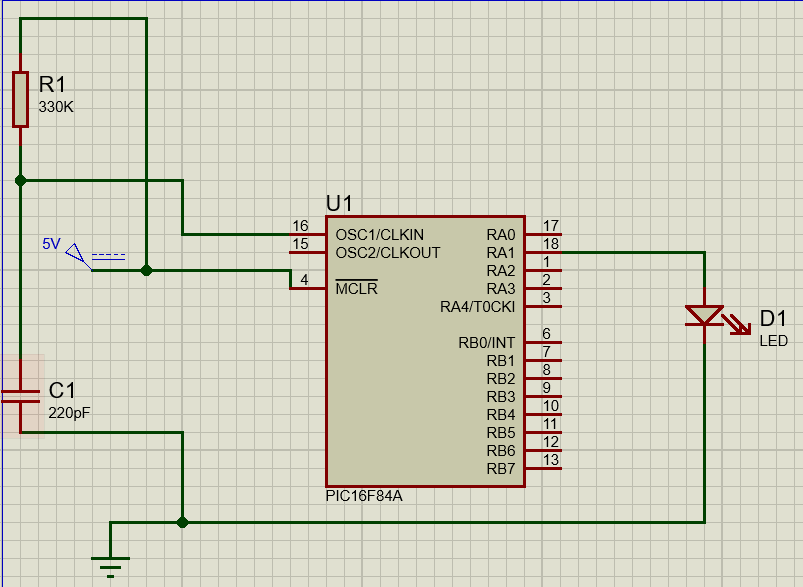
\includegraphics[width=0.3\paperwidth]{images/pic16f84a-assembly-sim.png}
        \caption{Circuito para PIC16F84A, programa ensamblador}
    \end{figure}

    \bigbreak

    Con la excepción de que varían algunas cosas en el simulador Proteus.
    Solo se fue capaz de agragar un PIC 16F84\textbf{A} el cual no cuenta con
    la terminar 14 para la alimentación y la 5 para tierra o $0V$.

    \section{Programa C}

    En esta sección se provee un programa escrito en lenguaje C para PIC16 de
    \textit{PIC1000: Getting Started with Writing C-Code for PIC16 and PIC18}
    \cite{microchip-c-program-2020}.

    \bigbreak

    El programa que se mostrará es sobre como configurar el microcontrolador
    para encender un LED cuando un usuario presione un botón. Por tanto, es
    parecido al programa desarrollado en ensamblador.

    \bigbreak

    Para esto, el usuario necesita identificar los pines del microcontrolador
    que van al LED del usuario y al botón. El programa es para el PIC18F47Q10
    (el cual no pertenece a la gama de entrada que se mencionó arriba) pero
    puede resultar útil al lector ya que es de la guía oficial la cual es
    para modelos PIC16 y PIC18.

    \begin{lstlisting}[language=C, caption=Encender el LED al presionar el
    botón (con unión de bit)]
    #include <xc.h>
    void main(void)
    {
        /* Configurar el pin RE0 como salida del LED */
        TRISEbits.TRISE0 = 0;
        /* Configurar el pin RE2 como entrada del boton */
        TRISEbits.TRISE2 = 1;
        /* Activar el buffer de entrada digital para el pin RE2 (boton) */
        ANSELEbits.ANSELE2 = 0;
        /* Activar el pull-up interno para el pin RE2 (boton)*/
        WPUEbits.WPUE2 = 1;

        /* Loop principal */
        while(1)
        {
            /* Si se presiona el boton (RE2 en alto) */
            if(PORTEbits.RE2)
            {
                /* Encender el LED (RE0 en alto) */
                LATEbits.LATE0 = 1;
            }
            else
            {
                /* Apagar el LED (RE0 bajo) */
                LATEbits.LATE0 = 0;
            }
        }
    }
\end{lstlisting}

Tener en cuenta la entrada (el botón) y la salida (el LED) al realizar el
circuito el cual va en el mismo estilo que el circuito presentado
anteriormente con el programa en ensamblador. Con este ejemplo se concluye la
sección del lenguaje C.

\section{Conclusión}

Se detalló brevemente sobre los microcontroladores PIC y la importancia que
tienen en la actualidad y han tenido en el pasado. Se presentaron dos
ejemplos de programas para microcontrolador PIC16 tanto en lenguaje
ensamblador como en lenguaje C y considerando a estos como la gama de entrada
que se ve más comúnmente.

\printbibliography

\end{document}
